%
% File acl2021.tex
%
%% Based on the style files for EMNLP 2020, which were
%% Based on the style files for ACL 2020, which were
%% Based on the style files for ACL 2018, NAACL 2018/19, which were
%% Based on the style files for ACL-2015, with some improvements
%%  taken from the NAACL-2016 style
%% Based on the style files for ACL-2014, which were, in turn,
%% based on ACL-2013, ACL-2012, ACL-2011, ACL-2010, ACL-IJCNLP-2009,
%% EACL-2009, IJCNLP-2008...
%% Based on the style files for EACL 2006 by 
%%e.agirre@ehu.es or Sergi.Balari@uab.es
%% and that of ACL 08 by Joakim Nivre and Noah Smith

\documentclass[11pt,a4paper]{article}
\usepackage[hyperref]{acl2021}
\usepackage{times}
\usepackage{latexsym}
\usepackage{amsmath}
\usepackage{graphicx}
\renewcommand{\UrlFont}{\ttfamily\small}

% This is not strictly necessary, and may be commented out,
% but it will improve the layout of the manuscript,
% and will typically save some space.
\usepackage{microtype}

\aclfinalcopy % Uncomment this line for the final submission
%\def\aclpaperid{***} %  Enter the acl Paper ID here

%\setlength\titlebox{5cm}
% You can expand the titlebox if you need extra space
% to show all the authors. Please do not make the titlebox
% smaller than 5cm (the original size); we will check this
% in the camera-ready version and ask you to change it back.

\newcommand\BibTeX{B\textsc{ib}\TeX}

\title{Generating Regex through Modern Architectural Optimizations}

\author{Kunal Agarwal \\
  University of California, Berkeley \\
  \texttt{kagarwal2@berkeley.edu} \\\And
  Parth Baokar \\
  University of California, Berkeley \\
  \texttt{parthbaokar@berkeley.edu} \\}

\date{}

\begin{document}
\maketitle
\begin{abstract}
% This document contains the instructions for preparing a manuscript for the proceedings of ACL-IJCNLP 2021.
% The document itself conforms to its own specifications, and is therefore an example of what your manuscript should look like.
% These instructions should be used for both papers submitted for review and for final versions of accepted papers.
% Authors are asked to conform to all the directions reported in this document.
This paper explores the latest research in the space of regular expression generation from text descriptions, as well as explores the popular models these regular expression generation models use. It then proceeds to propose a few enhancements that could be used to improve upon the most current models. The paper then explores preliminary attempts at implementing these proposals and reflects on what went wrong and what should be done for future work in this area.
\end{abstract}

% \section{Credits}
% DO WE NEED THIS? - KA

% This document has been adapted by Roberto Navigli
% from the instructions for earlier ACL, NAACL and EMNLP proceedings, including those for 
% EMNLP 2020 by Yulan He,
% ACL 2020 by Steven Bethard, Ryan Cotterrell and Rui Yan, 
% ACL 2019 by Douwe Kiela and Ivan Vuli\'{c},
% NAACL 2019 by Stephanie Lukin and Alla Roskovskaya, 
% ACL 2018 by Shay Cohen, Kevin Gimpel, and Wei Lu, 
% NAACL 2018 by Margaret Michell and Stephanie Lukin,
% 2017/2018 (NA)ACL bibtex suggestions from Jason Eisner,
% ACL 2017 by Dan Gildea and Min-Yen Kan, 
% NAACL 2017 by Margaret Mitchell, 
% ACL 2012 by Maggie Li and Michael White, 
% ACL 2010 by Jing-Shing Chang and Philipp Koehn, 
% ACL 2008 by Johanna D. Moore, Simone Teufel, James Allan, and Sadaoki Furui, 
% ACL 2005 by Hwee Tou Ng and Kemal Oflazer, 
% ACL 2002 by Eugene Charniak and Dekang Lin, 
% and earlier ACL and EACL formats written by several people, including
% John Chen, Henry S. Thompson and Donald Walker.
% Additional elements were taken from the formatting instructions of the \emph{International Joint Conference on Artificial Intelligence} and the \emph{Conference on Computer Vision and Pattern Recognition}.

\section{Introduction}

Regular expressions (Regex) are a fundamental part of the text processing and analysis toolkit. Regex is widely used in preprocessing steps for textual data from removing punctuation to input validation in form fields. Regular expressions offer a powerful syntax to abstract common patterns within text, but its expressiveness comes at the cost of a high learning curve. Small idiosyncrasies when creating Regex make it difficult for beginners to learn to build their own expressions, and can continue to be challenging for the experienced \cite{Friedl:02}. The consequences for incorrect regex can be drastic as well as failure in input validation can open applications to several security flaws. 

However, the mechanics of creating an expression through the combination of metacharacters, grouping characters, and ASCII characters are identical to that of the processes underlying word and sentence formation in natural language. Regex can be considered a language in and of itself, so it should be possible to parse specifications in English and synthesize regular expression that satisfies the constraints of the request in a process not unlike translation between two natural languages. A regex generator from natural language presents itself as a useful tool in education and engineering environments. New students can experiment with the generator to build an intuition for regex syntax and meaning, while experienced programmers can simplify the process of creating secure expressions in their production applications. 

In this work, we present new and updated approaches to generating regex through modern transformer architectures. These large language models could serve as ideal candidates for capturing the semantic nuance in translating regex. We pre-trained a new BERT model, ReBERTh, on a sizable corpus and used the embeddings to attempt to generate more accurate similarity scores for two regular expressions. We additionally fine-tuned a T5 transformer to directly translate queries into regex to hopefully take advantage of transfer learning for this difficult translation problem.

\section{Related Work}
There are two major approaches that have been taken in translating natural language queries into a corresponding regular expression: a syntactic or semantic approach. The syntactic approach frames this program synthesis question as a machine translation task; it optimizes an objective function that penalizes translations that are not syntactically equivalent (do not have the exact same characters). A semantic approach uses an objective function that encourages translations that have the same inherent meaning.

\subsection*{Sequence-to-Sequence Learning}

Many approaches in translation are based on a common deep learning architecture known as Seq2seq \cite{seq2seq}. Seq2seq models are characterized by their use of recurrent neural networks (RNN) with LSTM (Long Short-Term Memory) \cite{hochreiter1997long} cells. The Seq2seq framework uses an encoder-decoder architecture with two LSTMs: one to generate a fixed-dimensional embedding of a sequence, and another to decode the embedding into a target sequence. LSTMs are used to mitigate the effect of the vanishing gradient problem present in traditional RNNs and allow long term dependencies between several tokens in a sequence. Pairing the Seq2seq architecture with a global attention mechanism \cite{attention} enables better sequence embeddings by dynamically determining the importance of words across the whole sequence. 

\subsection*{Regex Neural Machine Translation}

The first attempts at generalized regex synthesis include a model called DeepRegex \cite{locascio-etal-2016-neural} that is directly based on Seq2seq. Optimal parameters for the underlying encoder and decoder architectures are found through maximum likelihood estimation (MLE). The MLE objective enforces syntactically equivalent expressions and discourages semantically equivalent expressions, leading to overall poorer performance.

However, by wrongfully penalizing correct expressions, syntactic translations approaches can often fail to capture the expressiveness of regular expressions. SemRegex \cite{zhong-etal-2018-semregex} relies on a semantics based approach to determine the correctness of a regular expression. The underlying model is still the same architecture used by DeepRegex, but instead SemRegex uses policy gradient methods \cite{Williams:92} to determine the gradient of a semantic based objective (as opposed to the MLE). Through the use of a reward function $r$, maximizing the objective function encourages semantic correctness \cite{zhong-etal-2018-semregex}. $r(\cdot)$ is defined as $1$ if the predicted regular expression is semantically equivalent with the label for the given natural language query (the ground truth), and $0$ otherwise. To determine if two regular expressions are semantically equivalent, \cite{zhong-etal-2018-semregex} converts the regular expressions to their minimum DFA (Deterministic Finite Automaton). If these minimum DFAs are equivalent, then the regular expressions themselves are equivalent. 

Since there are an infinite number of regular expressions that may have the same minimum DFA as the ground truth, \cite{zhong-etal-2018-semregex} utilizes Monte Carlo sampling to estimate the expected reward of the output of a model. This estimate is then used by the REINFORCE policy gradient model \cite{Williams:92} which utilizes a baseline of the mean reward of the samples to reduce variance. The final gradient estimate looks like the following: \begin{align*} \nabla_{\theta} & J(\theta) \approx \\ & \sum_{(S^{(i)}, R^{(i})} \sum_{j=1}^M \frac{1}{M}(r(R_j)-b) \nabla_{\theta}\log p_{\theta}(R_j | S^{(i)}) \end{align*}
for $R_1, ..., R_M$ where $R_i$ is a regular expression sampled from the model, and $b = \sum_{j^{\prime}}^M \frac{1}{M}r(R_{j^{\prime}})$ \cite{zhong-etal-2018-semregex}.

SoftRegex \cite{park-etal-2019-softregex} extends the work in SemRegex, specifically tackling the issue of computational feasibility. Determining the semantic equivalence of two regular expressions through conversion to DFAs is a known PSPACE-complete problem, and SemRegex's reward function relied on on this step. Furthermore, the reward function was limited in its expressiveness, only outputting a binary value which constrained its ability to describe a spectrum of similarity between two regular expressions. SoftRegex uses an LSTM-based neural network architecture, EQ\_Reg, to estimate the similarity between two regular expressions, assigning a probability of similarity between the expressions, the output of which is the value of the reward function. By softening for the comparison of two regular expressions, SoftRegex trades a negligent drop in performance while greatly speeding up training time \cite{park-etal-2019-softregex}. 

The newest regular expression generation model is TransRegex \cite{Li:2021}. The model uses a similar seq-to-seq model used in DeepRegex and SoftRegex, but adds a Regex Fixer to the end of the model as a second part of the regular expression generation process. Regular expressions generated by the seq-to-seq model may be slightly off, and so to fix these small errors, an algorithm called SYNCORR is introduced. This algorithm defines a neighborhood $N(r)$ where $r$ is the regular expression. It then finds a local maximum with respect to some reward function of the regular expressions in $N(r)$. The SYNCORR fixing algorithm combined with the previous successful seq-to-seq models outperforms all the other models available in current literature.

Other attempts at semantic generation involve the use of a sketch --- an intermediate representation of the regex encapsulating macroscopic structure and fragments, instead of focusing on specific syntax. SketchRegex \cite{sketchregex} parses natural language to generate sketches from the natural language descriptions and then uses a program synthesizer to construct the resulting regex. The parsers come in two varieties: a Seq2seq model similar to DeepRegex or a grammar-based parser. The different parsers allowed the model to be optimized accordingly for low-data scenarios or performance on large datasets.

\subsection*{Transformers}
Modern NLP models are based on transformer architectures \cite{Vaswani:2017} that make use of encoder-decoder blocks for sequence-to-sequence translation, but without the use of recurrent neural networks. Traditional RNN sequence-to-sequence models aim to encode bidirectional dependencies but still fall victim to forgetting due to the sequential nature of generating text.  Transformers instead rely heavily on self-attention blocks. Self-attention allows embeddings for words in a sequence to derive weighted contextual meaning from the rest of the sequence, importantly enabling the encoding of global dependencies. The attention is computed in an order-agnostic way, and therefore introduces an additional positional embedding layer to relate ordinal information to the attention blocks \cite{2020t5}. Two widely popular transformer models, BERT and T5, could have potential use-cases in machine translation.

BERT trains bidirectional representations using unlabeled text \cite{devlin-etal-2019-bert}. BERT has revolutionized the space of transformer architectures for language problems. BERT can be pre-trained on large natural language corpora, and then used to tokenize sentences and generate representations of the sentences. BERT derives its power by providing representations of tokens with strong contextual embeddings to be used in a variety of different problems, including generating regular expressions. However, BERT functions as an "encoder-only" architecture, being used to generate embeddings that can be used for downstream tasks, which makes it ideal for classification problems but may not be as powerful in end-to-end translation tasks.

T5 returned to the traditional transformer roots, reintroducing the encoder-decoder setup \cite{2020t5}. This architectural shift allowed transformer architecture to become generally applicable to all NLP tasks, by modeling all NLP problems as text-to-text tasks. Unlike BERT, this approach is conducive to solving machine translation tasks end-to-end which is natively a text-to-text task.

\section{Data}

% TODO Clean up section
The data we are using are mostly comprised of parallel corpora from previous works. There are three main datasets of interest: KB13 \cite{kushman-barzilay-2013-using}, NL-RX Turk and Synth \cite{locascio-etal-2016-neural}, and NL-RX pair data \cite{park-etal-2019-softregex}. The labeled pair data is especially important in the initial experiments for fine-tuning BERT for determining semantic equivalence of regular expressions. These regular expressions are randomly generated by creating and combining data in a tree form \cite{park-etal-2019-softregex} using a process similar to the creation of NL-RX Synth \cite{locascio-etal-2016-neural}, and then labels the pairs. This process is extended to provide additional regular expression data for pre-training BERT embeddings on the regex language. 

% Move from here, maybe to future work?
Two more recent datasets have been created for evaluating the generation of regex: StackOverflow \cite{sketchregex} and StructuredRegex \cite{structuredregex}. The StackOverflow and StructuredRegex add a significant amount of complexity in regular expressions compared to the previous three datasets that can be included as training and testing samples to better evaluate regex generation.

\section{Method}

We explored two avenues of incorporating transformer-based models for this translation task.

\subsection{Improving the EQ\_Reg Model}
The first was to improve upon on SoftRegex through architectural changes in computing the similarity score and optimization of the policy gradient and a different optimization to improve accuracy and increase speed.

The EQ\_Reg model receives two regular expressions as input and passes each two separate LSTM layers to generate a latent vector representation. The latent vectors are concatenated and passed through a series of fully connected layers to generate a similarity measurement between 0 and 1. Instead of using an RNN architecture to generate latent vector representations, we switch to a BERT model to generate the latent vectors. BERT embeddings generally outperforms RNNs on downstream tasks for longer sequences due to the additional information incorporated through a positional embedding layer \cite{devlin-etal-2019-bert}.

\textbf{ReBERTh:} We pre-trained a RoBERTa model and tokenizer at several different sizes \cite{roberta}. RoBERTa is an more optimized version of BERT, introducing several improvements such as removing the next sentence prediction objective, training on longer sequences, and dynamically changing masking patterns applied to the training set. These optimizations and more are why RoBERTa consistently performs better than BERT on common metrics \cite{roberta}.

In order to pretrain the BERT model, we generated a large corpus of approximately 300k regular expressions using a script provided in DeepRegex that was used to create the NL-RX-Synth dataset \cite{locascio-etal-2016-neural}. However since the regex is generated probabilistically with a relatively limited amount of tokens, we deduplicated the corpus to end up with approximately 60k expressions.

After creating the pretraining corpus, we trained four ReBERTh models with hyperparameters mimicking that of \texttt{bert-base}, \texttt{bert-medium}, \texttt{bert-small}, and \texttt{bert-mini}. Each model was trained for 5 epochs, ultimately limited by the amount of compute available. We used only \texttt{ReBERTh-base}

and model to replace the LSTM that SoftRegex uses. The SoftRegex model creates two LSTM models. Each regular expression in the pair is inputted to one of the LSTM models. The embeddings are concatenated together and then runs it through a few layers in a neural network, including a softmax layer, to get a label for whether or not the two regular expressions are equivalent or not. We've replaced the LSTM models with pretrained BERT models (bert-base-cased and bert-large-cased). In the pre-processing, we ensure we are tokenizing the regular expressions using our BERT model. We then create two BERT models, one for each regular expression in the pair. The BERT models will output representations of each of the regular expressions, which will be concatenated together and run through a linear layer and a softmax activation before being outputted. 

\textbf{Changing the Policy Gradient:} Now, looking at improving the REINFORCE algorithm, there are a number of different optimizations that could be used. One particular place to improve upon is using a more optimal baseline. While the average baseline used in SemRegex and SoftRegex generally works well \cite{Williams:92}, we want to explore how much of a performance improvement there would be if the optimal baseline is used. Looking at the gradient estimate defined earlier, we would want to replace the baseline $b$ with this optimal baseline instead of just using the average reward. The optimal baseline, as derived in \cite{peters-schaal-2008}, would look like: $$ b = \frac{\sum_{j=1}^M \frac{1}{M} (\nabla_{\theta} \log p_{\theta}(R_j | S^{(i)}))^2 r(R_j)}{\sum_{j=1}^M \frac{1}{M} (\nabla_{\theta} \log p_{\theta}(R_j | S^{(i)}))^2}$$ By using the optimal baseline, we are decreasing the variance of the policy gradient model without increasing bias, which should provide improvements in the performance of the model. However, after further research, we realized that this sort of optimization doesn't provide any reasonable improvement to the model \cite{peters-schaal-2008}. The vanilla policy gradient with the baseline set to be the average reward does well enough, without excessive computation. We decided not to follow the plan to optimize the baseline.

\subsection{Fine-tuning T5}

We fine-tuned a T5 model for regex translation. T5 is a large transformer model pretrained on large English corpora and is quite successful in transfer learning settings \cite{2020t5}. Additionally, it was already designed for sequence-to-sequence tasks, so it is an ideal candidate for syntactic translation similar to DeepRegex. , so after adjusting training data to fit the expected structure for translation tasks and fine-tuning the model, we can easily evaluate performance on the existing datasets.

% Write here the exact specifications of the T5 model we use
We used the \texttt{t5-base} model and tokenizer from \texttt{huggingface} \cite{2020t5}. In order to enable translation, we prepended each of the English queries from the evaluation datasets, KB13, NL-RX-Synth, and NL-RX-Turk with the task description "translate English to Regex:". The T5 model was separately fine-tuned on each dataset with a learning rate of $3 \cdot 10^{-4}$ for $35$ epochs. 

% Something more specific about T5

\section{Results and Analysis}



\begin{table}
\centering
\begin{tabular}{|c|c|c|c|}
\hline
 & \textbf{KB-13} & \textbf{NL-RX Turk} & \textbf{NL-RX Synth}\\
\hline
\textbf{T5} & 13.1\% & 5.6\% & 11.6\% \\
\textbf{ReBERTh} & 23.9\% & 20.8\% & 24.3\% \\
\textbf{DeepRegex} & 65.6\% & 58.2\% & 89.7\% \\
\textbf{SemRegex} & 77.5\% & 61.3\% & 90.2\% \\
\textbf{SoftRegex} & 78.2\% & 62.8\% & 91.4\% \\\hline
\end{tabular}
\caption{Accuracy for different models for each of the three different datasets \cite{park-etal-2019-softregex}.}\label{tab:accents}
\end{table}

\begin{table}
\centering
\begin{tabular}{|c|c|c|c|}
\hline
\textbf{Epoch} & \textbf{KB-13} & \textbf{NL-RX Turk} & \textbf{NL-RX Synth}\\
\hline
1 & 1.22  & 0.17 & 0.07 \\
6 & 0.24  & 0.07 & 0.01  \\
11 & 0.18  & 0.06 & 0.01  \\
16 & 0.17  & 0.06 & 0.01  \\
21 & 0.15 & 0.06 & 0.01  \\
26 & 0.15  & 0.06 & 0.01  \\
31 & 0.15  & 0.06 & 0.01 \\\hline
\end{tabular}
\caption{Validation Loss during the training of the T5 algorithm every 5th epoch for three different datasets.}\label{tab:accents}
\end{table}

\begin{table}
\centering
\begin{tabular}{|c|c|c|c|}
\hline
 & \textbf{KB-13} & \textbf{NL-RX Turk} & \textbf{NL-RX Synth}\\
\hline
\textbf{(1)} & 13.1\% & 5.6\% & 11.6\% \\
\textbf{(2)} & 29.9\% & 8.4\% & 24.4\% \\\hline
\end{tabular}
\caption{Accuracy comparison between the full dataset (1) and a subset of the dataset containing regular expressions of length less than 15 characters (2).}\label{tab:accents}
\end{table}

% TODO fix this section
\subsection*{Evaluating Performance}We then determined accuracy using the minimum DFA of each regular expression by comparing the gold regular expression's minimum DFA with the generated regular expression's minimum DFA. 

% TODO Clean up section
\subsection*{T5 Results and Analysis}
We split each dataset into three parts where 65\% of the data is used for training, 10\% is used for validation, and the rest is used as a test set. The T5 model is trained using the training data. At each epoch the model is evaluated on its performance using the validation set. The accuracy is then computed at the end of the $35$ epochs by running the model on the unseen data in the test set. We compare the minimum DFAs of both the generated regular expression and the gold regular expressions to determine if the generated regular expression is correct while computing the accuracy. As we see in Table 2, the validation loss for all three goes down as the training commences. However, as we see in Table 1, the accuracy of the model isn't great. While T5 does seem to train on regular expressions and is able to output correct regular expressions for a decent amount of unseen data, it does poorly overall and is not a great model to use for this translation task. We believe one of the reasons behind this is due to the fact that the T5 tokenizer is not optimized for regular expressions. Many characters important to regular expressions like \texttt{\textbackslash} or \texttt{\{ \}} are not showing up as tokens. In fact, they're replaced by the T5 tokenizer as unknown tokens. To fix this, we would train a T5 tokenizer using regular expression data. However, due to our lack of readily available GPU clusters, we were unable to perform this optimization. 

An interesting finding from our analysis of the T5 results shed light to an interesting pattern. We found that the model tended to do significantly better on regex data where the regular expression was shorter. In Table 3, you can see how the accuracy significantly improved when we restricted the data to only regular expressions with less than 15 characters. This seems to imply that the model does better when there are few characters. This could be a product of fewer epochs being used to train the model, or it could be the result of structure of the data we have at our disposal.

\subsection*{BERT Model Results and Analysis}


\begin{table}
\centering
\begin{tabular}{|c|c|c|c|c|}
\hline
\textbf{Step} & \textbf{base} & \textbf{medium} & \textbf{small} & \textbf{mini} \\
\hline
500 & 2.53  & 2.94 & 3.09 & 4.09 \\
1000 & 1.42  & 1.65 & 1.74 & 2.67 \\
1500 & 1.17  & 1.37 & 1.43 & 2.13 \\
2000 & 1.00  & 1.21 & 1.29 & 1.82 \\
2500 & 0.84 & 1.10 & 1.20 & 1.67 \\
3000 & 0.74  & 1.00 & 1.14 & 1.56 \\
3500 & 0.65  & 0.93 & 1.08 & 1.48 \\
4000 & 0.60  & 0.87 & 1.04 & 1.45 \\
4500 & 0.56  & 0.84 & 1.00 & 1.40 \\
5000 & 0.53  & 0.81 & 0.98 & 1.39 \\\hline
\end{tabular}
\caption{Training loss per training step for different BERT models trained to be used in reBERTh.}\label{tab:accents}
\end{table}

\begin{figure}
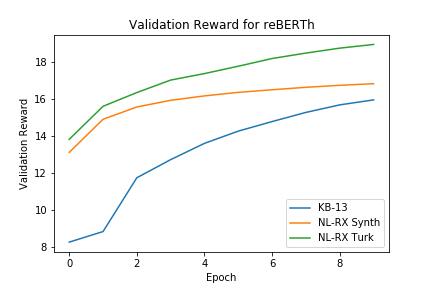
\includegraphics[width=8cm, height=6cm]{pic.png}
\caption{Validation Reward while running policy gradient on three different datasets}\label{tab:accents}
\end{figure}

We trained our BERT based model reBERTh... % TODO: Talk about what was done to train the model

One of the reasons why we believe the policy gradient algorithm which used reBERTh had its validation reward continue to go up while the accuracy stayed the same was due to the fact that the reBERTh model was not especially great. Even though the reBERTh model itself is poor at generating correct reward values, the policy gradient model would slowly be encouraged towards different paths for generating the regular expression by the flawed reward function, causing the validation reward to go up. However, these paths are still fundamentally flawed, and only entrench the naive classification done at the first epoch. As a result, the accuracy doesn't change as the policy gradient algorithm runs.

\section{Conclusion}

\section{Future Work}
One problem we had right from the start was the lack of available compute clusters to train these large complex models. We had to make do with the limited GPU resources on Google Colab. We tried to get around this by training our models for fewer epochs or on smaller datasets, or using models and tokenizers pretrained on smaller datasets. In any case, our models were never going to perform at its peak possible performance. In addition, due to the rate limiting Google Colab does on their GPU usage, we have fewer opportunities to run experiments. As a result, we are unable to fully do hyperparameter tuning to change things like the learning rate to improve the model. In the future, we hope to gain access to a GPU cluster to improve the models we discuss in this paper.



% Our preliminary experiment involved editing the SoftRegex code to replace the LSTMs with BERT models. We also edited how the model was tokenized by switching from a basic tokenizer to the BERT tokenizer. We were able to successfully implement it, but the model is infeasible to run, and could not be trained past two epochs on the data. Since BERT is trained on natural language expressions and we could not train for a significant number of epochs, this change provided no performance improvement.

% To follow-up with this attempt, we are planning on using a smaller BERT model in order to be able to complete the run successfully. We also plan on experimenting with the complexity of the neural network so see if that can improve the model. 

% The other optimization we proposed was to improve the baseline of the policy gradient algorithm, REINFORCE \cite{Williams:92}. 

% add Bert

% While testing the model with bert-mini and bert-small may provide an improvement since it may be much more computationally feasible to train for more epochs, this will just be used as a minor benchmark. The BERT models are all trained on natural language corpora that do not have much relation in the regular expression domain. We plan to use generated NL-RX data from DeepRegex scripts \cite{locascio-etal-2016-neural} to generate expression to pre-train a BERT model from scratch on regex. This allows a much greater degree of flexibility in using a simpler model architecture and limiting vocabulary. Regular expressions as a language are much simpler than natural languages that allows us to reasonably expect encodings with smaller models to perform well. Additionally, it can help significantly speed up pre-training and fine-tuning as computational feasibility of BERT is a concern. After pre-training BERT with new examples of regular expressions, we can fine-tune BERT as before to insert as the new EQ\_Reg model and evaluate its performance.




% \section{Evaluation Strategy}

% Most if not all of our data described above comes with labeled train and test data. After training the models, we will evaluate the accuracy on the StackOverflow, KB13, and NL-RX datasets in order to compare performance across as many previous models as possible. Most of the models studied evaluate their performance on KB13 and NL-RX datasets which means we do not have to re-evaluate DeepRegex, SemRegex, SoftRegex, SketchRegex, and TransRegex on any of these datasets. Performance is measured by DFA accuracy which checks whether the generated regex is semantically equivalent to the target regex rather requiring than exact syntactic equivalence.

% \paragraph{\LaTeX-specific details:}
% For an anonymized submission, ensure that {\small\verb|\aclfinalcopy|} at the top of this document is commented out, and that you have filled in the paper ID number (assigned during the submission process on softconf) where {\small\verb|***|} appears in the {\small\verb|\def\aclpaperid{***}|} definition at the top of this document.
% For a camera-ready submission, ensure that {\small\verb|\aclfinalcopy|} at the top of this document is not commented out.


% \section{Multiple Submission Policy}

% ACL-IJCNLP 2021 will not consider any paper that is under review in a journal or another conference at the time of submission, and submitted papers must not be submitted elsewhere during the ACL-IJCNLP 2021 review period. This policy covers all refereed and archival conferences and workshops (e.g., NAACL). The only exception is that a paper can be dual-submitted to both ACL-IJCNLP 2021 and an ACL-IJCNLP workshop. 

% In addition, we will not consider any paper that overlaps significantly in content or results with papers that will be (or have been) published elsewhere. 
% Authors submitting more than one paper to ACL-IJCNLP 2021 must ensure that their submissions do not overlap significantly ($>25$\%) with each other in content or results.

% \section{Formatting Instructions}

% Manuscripts must be in two-column format.
% Exceptions to the two-column format include the title, authors' names and complete addresses, which must be centered at the top of the first page, and any full-width figures or tables (see the guidelines in Section~\ref{ssec:title-authors}).
% \textbf{Type single-spaced.}
% Start all pages directly under the top margin.
% The manuscript should be printed single-sided and its length should not exceed the maximum page limit described in Section~\ref{sec:length}.
% Pages should be numbered in the version submitted for review, but \textbf{pages should not be numbered in the camera-ready version}.

% \paragraph{\LaTeX-specific details:}
% The style files will generate page numbers when {\small\verb|\aclfinalcopy|} is commented out, and remove them otherwise.


% \subsection{File Format}
% \label{sect:pdf}

% For the production of the electronic manuscript you must use Adobe's Portable Document Format (PDF).
% Please make sure that your PDF file includes all the necessary fonts (especially tree diagrams, symbols, and fonts with Asian characters).
% When you print or create the PDF file, there is usually an option in your printer setup to include none, all or just non-standard fonts.
% Please make sure that you select the option of including ALL the fonts.
% \textbf{Before sending it, test your PDF by printing it from a computer different from the one where it was created.}
% Moreover, some word processors may generate very large PDF files, where each page is rendered as an image.
% Such images may reproduce poorly.
% In this case, try alternative ways to obtain the PDF.
% One way on some systems is to install a driver for a postscript printer, send your document to the printer specifying ``Output to a file'', then convert the file to PDF.

% It is of utmost importance to specify the \textbf{A4 format} (21 cm x 29.7 cm) when formatting the paper.
% Print-outs of the PDF file on A4 paper should be identical to the hardcopy version.
% If you cannot meet the above requirements about the production of your electronic submission, please contact the publication chairs as soon as possible.

% \paragraph{\LaTeX-specific details:}
% PDF files are usually produced from \LaTeX{} using the \texttt{\small pdflatex} command.
% If your version of \LaTeX{} produces Postscript files, \texttt{\small ps2pdf} or \texttt{\small dvipdf} can convert these to PDF.
% To ensure A4 format in \LaTeX, use the command {\small\verb|\special{papersize=210mm,297mm}|}
% in the \LaTeX{} preamble (below the {\small\verb|\usepackage|} commands) and use \texttt{\small dvipdf} and/or \texttt{\small pdflatex}; or specify \texttt{\small -t a4} when working with \texttt{\small dvips}.

% \subsection{Layout}
% \label{ssec:layout}

% Format manuscripts two columns to a page, in the manner these
% instructions are formatted.
% The exact dimensions for a page on A4 paper are:

% \begin{itemize}
% \item Left and right margins: 2.5 cm
% \item Top margin: 2.5 cm
% \item Bottom margin: 2.5 cm
% \item Column width: 7.7 cm
% \item Column height: 24.7 cm
% \item Gap between columns: 0.6 cm
% \end{itemize}

% \noindent Papers should not be submitted on any other paper size.
% If you cannot meet the above requirements about the production of your electronic submission, please contact the publication chairs above as soon as possible.

% \subsection{Fonts}

% For reasons of uniformity, Adobe's \textbf{Times Roman} font should be used.
% If Times Roman is unavailable, you may use Times New Roman or \textbf{Computer Modern Roman}.

% Table~\ref{font-table} specifies what font sizes and styles must be used for each type of text in the manuscript.

% \begin{table}
% \centering
% \begin{tabular}{lrl}
% \hline \textbf{Type of Text} & \textbf{Font Size} & \textbf{Style} \\ \hline
% paper title & 15 pt & bold \\
% author names & 12 pt & bold \\
% author affiliation & 12 pt & \\
% the word ``Abstract'' & 12 pt & bold \\
% section titles & 12 pt & bold \\
% subsection titles & 11 pt & bold \\
% document text & 11 pt  &\\
% captions & 10 pt & \\
% abstract text & 10 pt & \\
% bibliography & 10 pt & \\
% footnotes & 9 pt & \\
% \hline
% \end{tabular}
% \caption{\label{font-table} Font guide. }
% \end{table}

% \paragraph{\LaTeX-specific details:}
% To use Times Roman in \LaTeX2e{}, put the following in the preamble:
% \begin{quote}
% \small
% \begin{verbatim}
% \usepackage{times}
% \usepackage{latexsym}
% \end{verbatim}
% \end{quote}


% \subsection{Ruler}
% A printed ruler (line numbers in the left and right margins of the article) should be presented in the version submitted for review, so that reviewers may comment on particular lines in the paper without circumlocution.
% The presence or absence of the ruler should not change the appearance of any other content on the page.
% The camera ready copy should not contain a ruler.

% \paragraph{Reviewers:}
% note that the ruler measurements may not align well with lines in the paper -- this turns out to be very difficult to do well when the paper contains many figures and equations, and, when done, looks ugly.
% In most cases one would expect that the approximate location will be adequate, although you can also use fractional references (\emph{e.g.}, this line ends at mark $295.5$).

% \paragraph{\LaTeX-specific details:}
% The style files will generate the ruler when {\small\verb|\aclfinalcopy|} is commented out, and remove it otherwise.

% \subsection{Title and Authors}
% \label{ssec:title-authors}

% Center the title, author's name(s) and affiliation(s) across both columns.
% Do not use footnotes for affiliations.
% Place the title centered at the top of the first page, in a 15-point bold font.
% Long titles should be typed on two lines without a blank line intervening.
% Put the title 2.5 cm from the top of the page, followed by a blank line, then the author's names(s), and the affiliation on the following line.
% Do not use only initials for given names (middle initials are allowed).
% Do not format surnames in all capitals (\emph{e.g.}, use ``Mitchell'' not ``MITCHELL'').
% Do not format title and section headings in all capitals except for proper names (such as ``BLEU'') that are
% conventionally in all capitals.
% The affiliation should contain the author's complete address, and if possible, an electronic mail address.

% The title, author names and addresses should be completely identical to those entered to the electronical paper submission website in order to maintain the consistency of author information among all publications of the conference.
% If they are different, the publication chairs may resolve the difference without consulting with you; so it is in your own interest to double-check that the information is consistent.

% Start the body of the first page 7.5 cm from the top of the page.
% \textbf{Even in the anonymous version of the paper, you should maintain space for names and addresses so that they will fit in the final (accepted) version.}


% \subsection{Abstract}
% Use two-column format when you begin the abstract.
% Type the abstract at the beginning of the first column.
% The width of the abstract text should be smaller than the
% width of the columns for the text in the body of the paper by 0.6 cm on each side.
% Center the word \textbf{Abstract} in a 12 point bold font above the body of the abstract.
% The abstract should be a concise summary of the general thesis and conclusions of the paper.
% It should be no longer than 200 words.
% The abstract text should be in 10 point font.

% \subsection{Text}
% Begin typing the main body of the text immediately after the abstract, observing the two-column format as shown in the present document.

% Indent 0.4 cm when starting a new paragraph.

% \subsection{Sections}

% Format section and subsection headings in the style shown on the present document.
% Use numbered sections (Arabic numerals) to facilitate cross references.
% Number subsections with the section number and the subsection number separated by a dot, in Arabic numerals.

% \subsection{Footnotes}
% Put footnotes at the bottom of the page and use 9 point font.
% They may be numbered or referred to by asterisks or other symbols.\footnote{This is how a footnote should appear.}
% Footnotes should be separated from the text by a line.\footnote{Note the line separating the footnotes from the text.}

% \subsection{Graphics}

% Place figures, tables, and photographs in the paper near where they are first discussed, rather than at the end, if possible.
% Wide illustrations may run across both columns.
% Color is allowed, but adhere to Section~\ref{ssec:accessibility}'s guidelines on accessibility.

% \paragraph{Captions:}
% Provide a caption for every illustration; number each one sequentially in the form:
% ``Figure 1. Caption of the Figure.''
% ``Table 1. Caption of the Table.''
% Type the captions of the figures and tables below the body, using 10 point text.
% Captions should be placed below illustrations.
% Captions that are one line are centered (see Table~\ref{font-table}).
% Captions longer than one line are left-aligned (see Table~\ref{tab:accents}).

% \begin{table}
% \centering
% \begin{tabular}{lc}
% \hline
% \textbf{Command} & \textbf{Output}\\
% \hline
% \verb|{\"a}| & {\"a} \\
% \verb|{\^e}| & {\^e} \\
% \verb|{\`i}| & {\`i} \\ 
% \verb|{\.I}| & {\.I} \\ 
% \verb|{\o}| & {\o} \\
% \verb|{\'u}| & {\'u}  \\ 
% \verb|{\aa}| & {\aa}  \\\hline
% \end{tabular}
% \begin{tabular}{lc}
% \hline
% \textbf{Command} & \textbf{Output}\\
% \hline
% \verb|{\c c}| & {\c c} \\ 
% \verb|{\u g}| & {\u g} \\ 
% \verb|{\l}| & {\l} \\ 
% \verb|{\~n}| & {\~n} \\ 
% \verb|{\H o}| & {\H o} \\ 
% \verb|{\v r}| & {\v r} \\ 
% \verb|{\ss}| & {\ss} \\
% \hline
% \end{tabular}
% \caption{Example commands for accented characters, to be used in, \emph{e.g.}, \BibTeX\ names.}\label{tab:accents}
% \end{table}

% \paragraph{\LaTeX-specific details:}
% The style files are compatible with the caption and subcaption packages; do not add optional arguments.
% \textbf{Do not override the default caption sizes.}


% \subsection{Hyperlinks}
% Within-document and external hyperlinks are indicated with Dark Blue text, Color Hex \#000099.

% \subsection{Citations}
% Citations within the text appear in parentheses as~\citep{Gusfield:97} or, if the author's name appears in the text itself, as \citet{Gusfield:97}.
% Append lowercase letters to the year in cases of ambiguities.  
% Treat double authors as in~\citep{Aho:72}, but write as in~\citep{Chandra:81} when more than two authors are involved. Collapse multiple citations as in~\citep{Gusfield:97,Aho:72}. 

% Refrain from using full citations as sentence constituents.
% Instead of
% \begin{quote}
%   ``\citep{Gusfield:97} showed that ...''
% \end{quote}
% write
% \begin{quote}
% ``\citet{Gusfield:97} showed that ...''
% \end{quote}

% \begin{table*}
% \centering
% \begin{tabular}{lll}
% \hline
% \textbf{Output} & \textbf{natbib command} & \textbf{Old ACL-style command}\\
% \hline
% \citep{Gusfield:97} & \small\verb|\citep| & \small\verb|\cite| \\
% \citealp{Gusfield:97} & \small\verb|\citealp| & no equivalent \\
% \citet{Gusfield:97} & \small\verb|\citet| & \small\verb|\newcite| \\
% \citeyearpar{Gusfield:97} & \small\verb|\citeyearpar| & \small\verb|\shortcite| \\
% \hline
% \end{tabular}
% \caption{\label{citation-guide}
% Citation commands supported by the style file.
% The style is based on the natbib package and supports all natbib citation commands.
% It also supports commands defined in previous ACL style files for compatibility.
% }
% \end{table*}

% \paragraph{\LaTeX-specific details:}
% Table~\ref{citation-guide} shows the syntax supported by the style files.
% We encourage you to use the natbib styles.
% You can use the command {\small\verb|\citet|} (cite in text) to get ``author (year)'' citations as in \citet{Gusfield:97}.
% You can use the command {\small\verb|\citep|} (cite in parentheses) to get ``(author, year)'' citations as in \citep{Gusfield:97}.
% You can use the command {\small\verb|\citealp|} (alternative cite without  parentheses) to get ``author year'' citations (which is useful for  using citations within parentheses, as in \citealp{Gusfield:97}).


% \subsection{References}
% Gather the full set of references together under the heading \textbf{References}; place the section before any Appendices. 
% Arrange the references alphabetically by first author, rather than by order of occurrence in the text.

% Provide as complete a citation as possible, using a consistent format, such as the one for \emph{Computational Linguistics\/} or the one in the  \emph{Publication Manual of the American 
% Psychological Association\/}~\citep{APA:83}.
% Use full names for authors, not just initials.

% Submissions should accurately reference prior and related work, including code and data.
% If a piece of prior work appeared in multiple venues, the version that appeared in a refereed, archival venue should be referenced.
% If multiple versions of a piece of prior work exist, the one used by the authors should be referenced.
% Authors should not rely on automated citation indices to provide accurate references for prior and related work.

% The following text cites various types of articles so that the references section of the present document will include them.
% \begin{itemize}
% \item Example article in journal: \citep{Ando2005}.
% \item Example article in proceedings, with location: \citep{borschinger-johnson-2011-particle}.
% \item Example article in proceedings, without location: \citep{andrew2007scalable}.
% \item Example arxiv paper: \citep{rasooli-tetrault-2015}. 
% \end{itemize}


% \paragraph{\LaTeX-specific details:}
% The \LaTeX{} and Bib\TeX{} style files provided roughly follow the American Psychological Association format.
% If your own bib file is named \texttt{\small acl2021.bib}, then placing the following before any appendices in your \LaTeX{}  file will generate the references section for you:
% \begin{quote}\small
% \verb|\bibliographystyle{acl_natbib}|\\
% \verb|\bibliography{acl2021}|
% \end{quote}

% You can obtain the complete ACL Anthology as a Bib\TeX\ file from \url{https://aclweb.org/anthology/anthology.bib.gz}.
% To include both the anthology and your own bib file, use the following instead of the above.
% \begin{quote}\small
% \verb|\bibliographystyle{acl_natbib}|\\
% \verb|\bibliography{anthology,acl2021}|
% \end{quote}


% \subsection{Digital Object Identifiers}
% As part of our work to make ACL materials more widely used and cited outside of our discipline, ACL has registered as a CrossRef member, as a registrant of Digital Object Identifiers (DOIs), the standard for registering permanent URNs for referencing scholarly materials.

% All camera-ready references are required to contain the appropriate DOIs (or, as a second resort, the hyperlinked ACL Anthology Identifier) to all cited works.
% Appropriate records should be found for most materials in the current ACL Anthology at \url{http://aclanthology.info/}.
% As examples, we cite \citep{goodman-etal-2016-noise} to show you how papers with a DOI will appear in the bibliography.
% We cite \citep{harper-2014-learning} to show how papers without a DOI but with an ACL Anthology Identifier will appear in the bibliography.

% \paragraph{\LaTeX-specific details:}
% Please ensure that you use Bib\TeX\ records that contain DOI or URLs for any of the ACL materials that you reference.
% If the Bib\TeX{} file contains DOI fields, the paper title in the references section will appear as a hyperlink to the DOI, using the hyperref \LaTeX{} package.


% \section{Supplementary Materials}
% \label{sec:supplementary}

% Supplementary material may report preprocessing decisions, model parameters, and other details necessary for the replication of the experiments reported in the paper.
% Seemingly small preprocessing decisions can sometimes make a large difference in performance, so it is crucial to record such decisions to precisely characterize state-of-the-art methods. 

% Nonetheless, supplementary material should be supplementary (rather than central) to the paper.
% \textbf{Submissions that misuse the supplementary material may be rejected without review.}
% Supplementary material may include explanations or details of proofs or derivations that do not fit into the paper, lists of
% features or feature templates, sample inputs and outputs for a system, hyperparameter values, pseudo-code or source code, and data.

% The paper should not rely on the supplementary material: while the paper may refer to and cite the supplementary material and the supplementary material will be available to the reviewers, they will not be asked to review the supplementary material.

% Supplementary material can be uploaded as up to three separate files: a single appendix file in PDF format, a single .tgz or .zip archive containing software, and/or a single .tgz or .zip archive containing data.



% \subsection{Appendices}
% \label{sec:appendix}
% Appendices are material that can be read, and include lemmas, formulas, proofs, and tables that are not critical to the reading and understanding of the paper. 
% In the submitted version, appendices should be uploaded as a separate file. \textbf{Submissions which include appendices in the main paper will be rejected without review.} In the camera ready version, instead, appendices should directly follow the text and the references. 

% \paragraph{\LaTeX-specific details:}
% In your camera ready version use {\small\verb|\appendix|} before any appendix section to switch the section numbering over to letters.

% \subsection{Software and Data}
% \label{sec:software_and_data}
% Submissions may include software and data used in the work and described in the paper.
% Any accompanying software and/or data should include licenses and documentation of research review as appropriate.

% \section{Accessibility}
% \label{ssec:accessibility}

% In an effort to accommodate people who are color-blind (as well as those printing to paper), grayscale readability is strongly encouraged.
% Color is not forbidden, but authors should ensure that tables and figures do not rely solely on color to convey critical distinctions.
% A simple criterion:
% All curves and points in your figures should be clearly distinguishable without color.

% \section{Translation of non-English Terms}

% It is also advised to supplement non-English characters and terms with appropriate transliterations and/or translations since not all readers understand all such characters and terms.
% Inline transliteration or translation can be represented in the order of:
% \begin{center}
% \begin{tabular}{c}
% original-form \\
% transliteration \\
% ``translation''
% \end{tabular}
% \end{center}

% \section{\LaTeX{} Compilation Issues}
% You may encounter the following error during compilation: 
% \begin{quote}
% {\small\verb|\pdfendlink|} ended up in different nesting level than {\small\verb|\pdfstartlink|}.
% \end{quote}
% This happens when \texttt{\small pdflatex} is used and a citation splits across a page boundary.
% To fix this, the style file contains a patch consisting of two lines:
% (1) {\small\verb|\RequirePackage{etoolbox}|} (line 455 in \texttt{\small acl2021.sty}), and
% (2) A long line below (line 456 in \texttt{\small acl2021.sty}).

% If you still encounter compilation issues even with the patch enabled, disable the patch by commenting the two lines, and then disable the \texttt{\small hyperref} package by loading the style file with the \texttt{\small nohyperref} option:

% \noindent
% {\small\verb|\usepackage[nohyperref]{acl2021}|}

% \noindent
% Then recompile, find the problematic citation, and rewrite the sentence containing the citation. (See, {\em e.g.}, \url{http://tug.org/errors.html})

% \section*{Acknowledgments}

% We'd like to acknowledge Professor David Bamman for his insight on this project proposal.

\bibliographystyle{acl_natbib}
\bibliography{anthology,acl2021}

%\appendix



\end{document}
